\documentclass[twoside]{book}

% Packages required by doxygen
\usepackage{fixltx2e}
\usepackage{calc}
\usepackage{doxygen}
\usepackage[export]{adjustbox} % also loads graphicx
\usepackage{graphicx}
\usepackage[utf8]{inputenc}
\usepackage{makeidx}
\usepackage{multicol}
\usepackage{multirow}
\PassOptionsToPackage{warn}{textcomp}
\usepackage{textcomp}
\usepackage[nointegrals]{wasysym}
\usepackage[table]{xcolor}

% Font selection
\usepackage[T1]{fontenc}
\usepackage[scaled=.90]{helvet}
\usepackage{courier}
\usepackage{amssymb}
\usepackage{sectsty}
\renewcommand{\familydefault}{\sfdefault}
\allsectionsfont{%
  \fontseries{bc}\selectfont%
  \color{darkgray}%
}
\renewcommand{\DoxyLabelFont}{%
  \fontseries{bc}\selectfont%
  \color{darkgray}%
}
\newcommand{\+}{\discretionary{\mbox{\scriptsize$\hookleftarrow$}}{}{}}

% Page & text layout
\usepackage{geometry}
\geometry{%
  a4paper,%
  top=2.5cm,%
  bottom=2.5cm,%
  left=2.5cm,%
  right=2.5cm%
}
\tolerance=750
\hfuzz=15pt
\hbadness=750
\setlength{\emergencystretch}{15pt}
\setlength{\parindent}{0cm}
\setlength{\parskip}{3ex plus 2ex minus 2ex}
\makeatletter
\renewcommand{\paragraph}{%
  \@startsection{paragraph}{4}{0ex}{-1.0ex}{1.0ex}{%
    \normalfont\normalsize\bfseries\SS@parafont%
  }%
}
\renewcommand{\subparagraph}{%
  \@startsection{subparagraph}{5}{0ex}{-1.0ex}{1.0ex}{%
    \normalfont\normalsize\bfseries\SS@subparafont%
  }%
}
\makeatother

% Headers & footers
\usepackage{fancyhdr}
\pagestyle{fancyplain}
\fancyhead[LE]{\fancyplain{}{\bfseries\thepage}}
\fancyhead[CE]{\fancyplain{}{}}
\fancyhead[RE]{\fancyplain{}{\bfseries\leftmark}}
\fancyhead[LO]{\fancyplain{}{\bfseries\rightmark}}
\fancyhead[CO]{\fancyplain{}{}}
\fancyhead[RO]{\fancyplain{}{\bfseries\thepage}}
\fancyfoot[LE]{\fancyplain{}{}}
\fancyfoot[CE]{\fancyplain{}{}}
\fancyfoot[RE]{\fancyplain{}{\bfseries\scriptsize Generated by Doxygen }}
\fancyfoot[LO]{\fancyplain{}{\bfseries\scriptsize Generated by Doxygen }}
\fancyfoot[CO]{\fancyplain{}{}}
\fancyfoot[RO]{\fancyplain{}{}}
\renewcommand{\footrulewidth}{0.4pt}
\renewcommand{\chaptermark}[1]{%
  \markboth{#1}{}%
}
\renewcommand{\sectionmark}[1]{%
  \markright{\thesection\ #1}%
}

% Indices & bibliography
\usepackage{natbib}
\usepackage[titles]{tocloft}
\setcounter{tocdepth}{3}
\setcounter{secnumdepth}{5}
\makeindex

% Hyperlinks (required, but should be loaded last)
\usepackage{ifpdf}
\ifpdf
  \usepackage[pdftex,pagebackref=true]{hyperref}
\else
  \usepackage[ps2pdf,pagebackref=true]{hyperref}
\fi
\hypersetup{%
  colorlinks=true,%
  linkcolor=blue,%
  citecolor=blue,%
  unicode%
}

% Custom commands
\newcommand{\clearemptydoublepage}{%
  \newpage{\pagestyle{empty}\cleardoublepage}%
}

\usepackage{caption}
\captionsetup{labelsep=space,justification=centering,font={bf},singlelinecheck=off,skip=4pt,position=top}

%===== C O N T E N T S =====

\begin{document}

% Titlepage & ToC
\hypersetup{pageanchor=false,
             bookmarksnumbered=true,
             pdfencoding=unicode
            }
\pagenumbering{alph}
\begin{titlepage}
\vspace*{7cm}
\begin{center}%
{\Large date\+\_\+custom\+\_\+class }\\
\vspace*{1cm}
{\large Generated by Doxygen 1.8.13}\\
\end{center}
\end{titlepage}
\clearemptydoublepage
\pagenumbering{roman}
\tableofcontents
\clearemptydoublepage
\pagenumbering{arabic}
\hypersetup{pageanchor=true}

%--- Begin generated contents ---
\chapter{Class Index}
\section{Class List}
Here are the classes, structs, unions and interfaces with brief descriptions\+:\begin{DoxyCompactList}
\item\contentsline{section}{\hyperlink{classAnimal}{Animal} }{\pageref{classAnimal}}{}
\item\contentsline{section}{\hyperlink{classDangerousSnake}{Dangerous\+Snake} }{\pageref{classDangerousSnake}}{}
\item\contentsline{section}{\hyperlink{classDog}{Dog} }{\pageref{classDog}}{}
\item\contentsline{section}{\hyperlink{classNonDangerousSnake}{Non\+Dangerous\+Snake} }{\pageref{classNonDangerousSnake}}{}
\item\contentsline{section}{\hyperlink{structPython}{Python} }{\pageref{structPython}}{}
\item\contentsline{section}{\hyperlink{classSnake}{Snake} }{\pageref{classSnake}}{}
\end{DoxyCompactList}

\chapter{File Index}
\section{File List}
Here is a list of all documented files with brief descriptions\+:\begin{DoxyCompactList}
\item\contentsline{section}{/home/w-\/wilson/\+D\+S\+S\+C/first\+\_\+year/\+A\+P/advanced\+\_\+programming-\/2018-\/19/exercises/c++/04\+\_\+custom\+\_\+types/date/include/\hyperlink{date_8h}{date.\+h} \\*Declaration of \hyperlink{class_date}{Date} class }{\pageref{date_8h}}{}
\item\contentsline{section}{\hyperlink{date_8cc}{date.\+cc} \\*Implementation of the \hyperlink{class_date}{Date} class }{\pageref{date_8cc}}{}
\item\contentsline{section}{\hyperlink{main_8cc}{main.\+cc} \\*Tests the \hyperlink{class_date}{Date} class }{\pageref{main_8cc}}{}
\end{DoxyCompactList}

\chapter{Class Documentation}
\hypertarget{class_date}{}\section{Date Class Reference}
\label{class_date}\index{Date@{Date}}


Implement a date class.  




{\ttfamily \#include $<$date.\+h$>$}

\subsection*{Public Member Functions}
\begin{DoxyCompactItemize}
\item 
\mbox{\Hypertarget{class_date_a38b18986a934a931bcef3979697aa871}\label{class_date_a38b18986a934a931bcef3979697aa871}} 
unsigned int \hyperlink{class_date_a38b18986a934a931bcef3979697aa871}{day} () const
\begin{DoxyCompactList}\small\item\em Returns the value of the day variable. \end{DoxyCompactList}\item 
\mbox{\Hypertarget{class_date_a71889264c9f704db5a6e515f0739026e}\label{class_date_a71889264c9f704db5a6e515f0739026e}} 
\hyperlink{date_8h_a674553c60dd4ed7297e6c18d8139e067}{m\+\_\+enum} \hyperlink{class_date_a71889264c9f704db5a6e515f0739026e}{month} () const
\begin{DoxyCompactList}\small\item\em Returns the value of the month variable. \end{DoxyCompactList}\item 
\mbox{\Hypertarget{class_date_adb59de8d1ac3b04cbd57be3b551be2dc}\label{class_date_adb59de8d1ac3b04cbd57be3b551be2dc}} 
int \hyperlink{class_date_adb59de8d1ac3b04cbd57be3b551be2dc}{year} () const
\begin{DoxyCompactList}\small\item\em Returns the value of the year variable. \end{DoxyCompactList}\item 
\mbox{\Hypertarget{class_date_a038ecf65e8734086f8df30659f770cc2}\label{class_date_a038ecf65e8734086f8df30659f770cc2}} 
\hyperlink{class_date_a038ecf65e8734086f8df30659f770cc2}{Date} (unsigned int \+\_\+d, \hyperlink{date_8h_a674553c60dd4ed7297e6c18d8139e067}{m\+\_\+enum} \+\_\+m, int \+\_\+y)
\begin{DoxyCompactList}\small\item\em \hyperlink{class_date}{Date} constructor. \end{DoxyCompactList}\item 
bool \hyperlink{class_date_af12996155259f3fb64206bf250d50e10}{is\+\_\+leap} ()
\begin{DoxyCompactList}\small\item\em Checks if the year is leap. \end{DoxyCompactList}\item 
void \hyperlink{class_date_a1060f2334b942a33f16e76471225d0db}{add\+\_\+day} ()
\begin{DoxyCompactList}\small\item\em Adds a single day to the current date. \end{DoxyCompactList}\item 
void \hyperlink{class_date_a6bd05d49058041113ee34870a1268f2c}{add\+\_\+days} (const int n)
\begin{DoxyCompactList}\small\item\em Adds multiple days. \end{DoxyCompactList}\end{DoxyCompactItemize}


\subsection{Detailed Description}
Implement a date class. 

Contains function to add days and check if a year is leap 

\subsection{Member Function Documentation}
\mbox{\Hypertarget{class_date_a1060f2334b942a33f16e76471225d0db}\label{class_date_a1060f2334b942a33f16e76471225d0db}} 
\index{Date@{Date}!add\+\_\+day@{add\+\_\+day}}
\index{add\+\_\+day@{add\+\_\+day}!Date@{Date}}
\subsubsection{\texorpdfstring{add\+\_\+day()}{add\_day()}}
{\footnotesize\ttfamily void Date\+::add\+\_\+day (\begin{DoxyParamCaption}{ }\end{DoxyParamCaption})}



Adds a single day to the current date. 

Adds a single day checking if the month or the year needs to advance as well. 
\begin{DoxyParams}{Parameters}
{\em none} & \\
\hline
\end{DoxyParams}
\begin{DoxyReturn}{Returns}
none 
\end{DoxyReturn}
\mbox{\Hypertarget{class_date_a6bd05d49058041113ee34870a1268f2c}\label{class_date_a6bd05d49058041113ee34870a1268f2c}} 
\index{Date@{Date}!add\+\_\+days@{add\+\_\+days}}
\index{add\+\_\+days@{add\+\_\+days}!Date@{Date}}
\subsubsection{\texorpdfstring{add\+\_\+days()}{add\_days()}}
{\footnotesize\ttfamily void Date\+::add\+\_\+days (\begin{DoxyParamCaption}\item[{const int}]{n }\end{DoxyParamCaption})}



Adds multiple days. 

Calls \hyperlink{class_date_a1060f2334b942a33f16e76471225d0db}{add\+\_\+day()} n times. 
\begin{DoxyParams}{Parameters}
{\em n} & number of days to e added \\
\hline
\end{DoxyParams}
\begin{DoxyReturn}{Returns}
none 
\end{DoxyReturn}
\mbox{\Hypertarget{class_date_af12996155259f3fb64206bf250d50e10}\label{class_date_af12996155259f3fb64206bf250d50e10}} 
\index{Date@{Date}!is\+\_\+leap@{is\+\_\+leap}}
\index{is\+\_\+leap@{is\+\_\+leap}!Date@{Date}}
\subsubsection{\texorpdfstring{is\+\_\+leap()}{is\_leap()}}
{\footnotesize\ttfamily bool Date\+::is\+\_\+leap (\begin{DoxyParamCaption}{ }\end{DoxyParamCaption})}



Checks if the year is leap. 

Returns True if the year is divisible by 4 or by 400 
\begin{DoxyParams}{Parameters}
{\em none} & \\
\hline
\end{DoxyParams}
\begin{DoxyReturn}{Returns}
bool 
\end{DoxyReturn}


The documentation for this class was generated from the following files\+:\begin{DoxyCompactItemize}
\item 
/home/w-\/wilson/\+D\+S\+S\+C/first\+\_\+year/\+A\+P/advanced\+\_\+programming-\/2018-\/19/exercises/c++/04\+\_\+custom\+\_\+types/date/include/\hyperlink{date_8h}{date.\+h}\item 
\hyperlink{date_8cc}{date.\+cc}\end{DoxyCompactItemize}

\hypertarget{struct_invalid__day}{}\section{Invalid\+\_\+day Struct Reference}
\label{struct_invalid__day}\index{Invalid\+\_\+day@{Invalid\+\_\+day}}


Struct for exceptions regarding incorrect number of days per month.  




{\ttfamily \#include $<$date.\+h$>$}

\subsection*{Public Member Functions}
\begin{DoxyCompactItemize}
\item 
\mbox{\Hypertarget{struct_invalid__day_a27d2655de2518653ecf8b6e54505f3c8}\label{struct_invalid__day_a27d2655de2518653ecf8b6e54505f3c8}} 
{\bfseries Invalid\+\_\+day} (const std\+::string \&s)
\end{DoxyCompactItemize}
\subsection*{Public Attributes}
\begin{DoxyCompactItemize}
\item 
\mbox{\Hypertarget{struct_invalid__day_a2c5d881f7f92a74c8f323350271f5ecb}\label{struct_invalid__day_a2c5d881f7f92a74c8f323350271f5ecb}} 
std\+::string {\bfseries message}
\end{DoxyCompactItemize}


\subsection{Detailed Description}
Struct for exceptions regarding incorrect number of days per month. 

The documentation for this struct was generated from the following files\+:\begin{DoxyCompactItemize}
\item 
/home/w-\/wilson/\+D\+S\+S\+C/first\+\_\+year/\+A\+P/advanced\+\_\+programming-\/2018-\/19/exercises/c++/04\+\_\+custom\+\_\+types/date/include/\hyperlink{date_8h}{date.\+h}\item 
\hyperlink{date_8cc}{date.\+cc}\end{DoxyCompactItemize}

\chapter{File Documentation}
\hypertarget{date_8h}{}\section{/home/w-\/wilson/\+D\+S\+S\+C/first\+\_\+year/\+A\+P/advanced\+\_\+programming-\/2018-\/19/exercises/c++/04\+\_\+custom\+\_\+types/date/include/date.h File Reference}
\label{date_8h}\index{/home/w-\/wilson/\+D\+S\+S\+C/first\+\_\+year/\+A\+P/advanced\+\_\+programming-\/2018-\/19/exercises/c++/04\+\_\+custom\+\_\+types/date/include/date.\+h@{/home/w-\/wilson/\+D\+S\+S\+C/first\+\_\+year/\+A\+P/advanced\+\_\+programming-\/2018-\/19/exercises/c++/04\+\_\+custom\+\_\+types/date/include/date.\+h}}


Declaration of \hyperlink{class_date}{Date} class.  


{\ttfamily \#include $<$map$>$}\newline
{\ttfamily \#include $<$iostream$>$}\newline
{\ttfamily \#include $<$string$>$}\newline
Include dependency graph for date.\+h\+:\nopagebreak
\begin{figure}[H]
\begin{center}
\leavevmode
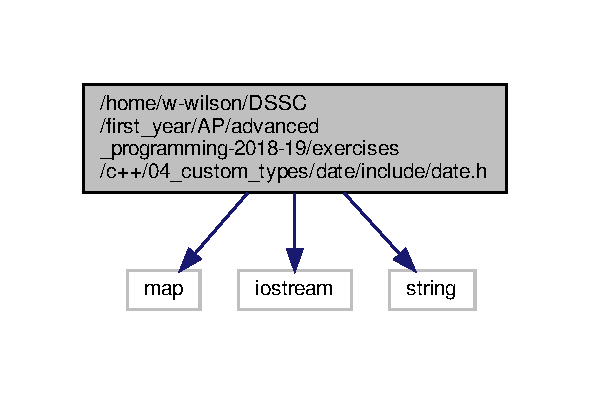
\includegraphics[width=283pt]{date_8h__incl}
\end{center}
\end{figure}
This graph shows which files directly or indirectly include this file\+:\nopagebreak
\begin{figure}[H]
\begin{center}
\leavevmode
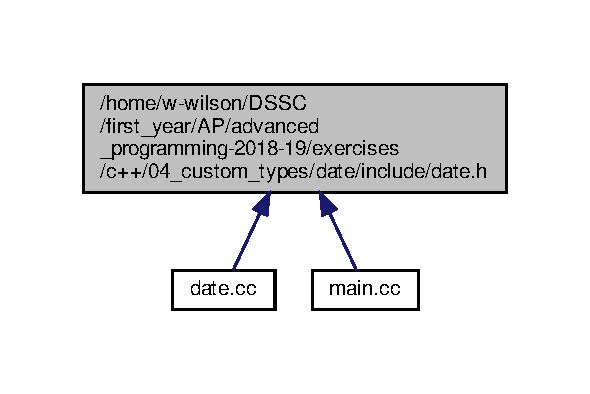
\includegraphics[width=283pt]{date_8h__dep__incl}
\end{center}
\end{figure}
\subsection*{Classes}
\begin{DoxyCompactItemize}
\item 
struct \hyperlink{struct_invalid__day}{Invalid\+\_\+day}
\begin{DoxyCompactList}\small\item\em Struct for exceptions regarding incorrect number of days per month. \end{DoxyCompactList}\item 
class \hyperlink{class_date}{Date}
\begin{DoxyCompactList}\small\item\em Implement a date class. \end{DoxyCompactList}\end{DoxyCompactItemize}
\subsection*{Enumerations}
\begin{DoxyCompactItemize}
\item 
\mbox{\Hypertarget{date_8h_a674553c60dd4ed7297e6c18d8139e067}\label{date_8h_a674553c60dd4ed7297e6c18d8139e067}} 
enum \hyperlink{date_8h_a674553c60dd4ed7297e6c18d8139e067}{m\+\_\+enum} \{ \newline
{\bfseries jan} = 1, 
{\bfseries feb}, 
{\bfseries mar}, 
{\bfseries apr}, 
\newline
{\bfseries may}, 
{\bfseries jun}, 
{\bfseries jul}, 
{\bfseries aug}, 
\newline
{\bfseries sep}, 
{\bfseries oct}, 
{\bfseries nov}, 
{\bfseries dec}
 \}\begin{DoxyCompactList}\small\item\em Enum Class cointaining the months of a year. \end{DoxyCompactList}
\end{DoxyCompactItemize}
\subsection*{Functions}
\begin{DoxyCompactItemize}
\item 
\mbox{\Hypertarget{date_8h_a1862604492a841a6b98e1a3061d95b96}\label{date_8h_a1862604492a841a6b98e1a3061d95b96}} 
std\+::ostream \& {\bfseries operator$<$$<$} (std\+::ostream \&os, const \hyperlink{class_date}{Date} \&date)
\item 
\mbox{\Hypertarget{date_8h_a27425be265a0cc57e4f731825154ec4d}\label{date_8h_a27425be265a0cc57e4f731825154ec4d}} 
bool {\bfseries operator==} (const \hyperlink{class_date}{Date} \&lhs, const \hyperlink{class_date}{Date} \&rhs)
\item 
\mbox{\Hypertarget{date_8h_ad12683e4457513f4f834e13c4e7f72f8}\label{date_8h_ad12683e4457513f4f834e13c4e7f72f8}} 
bool {\bfseries operator!=} (const \hyperlink{class_date}{Date} \&lhs, const \hyperlink{class_date}{Date} \&rhs)
\end{DoxyCompactItemize}


\subsection{Detailed Description}
Declaration of \hyperlink{class_date}{Date} class. 

\begin{DoxyAuthor}{Author}
Patrick Indri 
\end{DoxyAuthor}
\begin{DoxyDate}{Date}
14/01/19 
\end{DoxyDate}

\hypertarget{date_8cc}{}\section{date.\+cc File Reference}
\label{date_8cc}\index{date.\+cc@{date.\+cc}}


implementation of the \hyperlink{class_date}{Date} class  


{\ttfamily \#include $<$iostream$>$}\newline
{\ttfamily \#include $<$map$>$}\newline
{\ttfamily \#include \char`\"{}date.\+h\char`\"{}}\newline
Include dependency graph for date.\+cc\+:\nopagebreak
\begin{figure}[H]
\begin{center}
\leavevmode
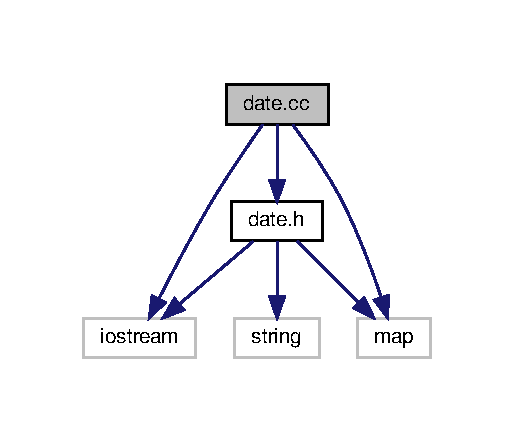
\includegraphics[width=247pt]{date_8cc__incl}
\end{center}
\end{figure}
\subsection*{Functions}
\begin{DoxyCompactItemize}
\item 
\mbox{\Hypertarget{date_8cc_a1862604492a841a6b98e1a3061d95b96}\label{date_8cc_a1862604492a841a6b98e1a3061d95b96}} 
std\+::ostream \& {\bfseries operator$<$$<$} (std\+::ostream \&os, const \hyperlink{class_date}{Date} \&date)
\item 
\mbox{\Hypertarget{date_8cc_a27425be265a0cc57e4f731825154ec4d}\label{date_8cc_a27425be265a0cc57e4f731825154ec4d}} 
bool {\bfseries operator==} (const \hyperlink{class_date}{Date} \&lhs, const \hyperlink{class_date}{Date} \&rhs)
\item 
\mbox{\Hypertarget{date_8cc_ad12683e4457513f4f834e13c4e7f72f8}\label{date_8cc_ad12683e4457513f4f834e13c4e7f72f8}} 
bool {\bfseries operator!=} (const \hyperlink{class_date}{Date} \&lhs, const \hyperlink{class_date}{Date} \&rhs)
\end{DoxyCompactItemize}


\subsection{Detailed Description}
implementation of the \hyperlink{class_date}{Date} class 

\begin{DoxyAuthor}{Author}
Patrick Indri 
\end{DoxyAuthor}
\begin{DoxyDate}{Date}
14/01/19 
\end{DoxyDate}

\hypertarget{main_8cc}{}\section{main.\+cc File Reference}
\label{main_8cc}\index{main.\+cc@{main.\+cc}}


Tests the \hyperlink{class_date}{Date} class.  


{\ttfamily \#include $<$iostream$>$}\newline
{\ttfamily \#include $<$map$>$}\newline
{\ttfamily \#include \char`\"{}date.\+h\char`\"{}}\newline
Include dependency graph for main.\+cc\+:\nopagebreak
\begin{figure}[H]
\begin{center}
\leavevmode
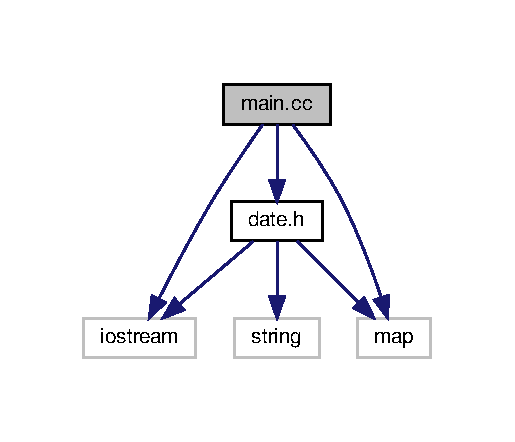
\includegraphics[width=247pt]{main_8cc__incl}
\end{center}
\end{figure}
\subsection*{Functions}
\begin{DoxyCompactItemize}
\item 
\mbox{\Hypertarget{main_8cc_ae66f6b31b5ad750f1fe042a706a4e3d4}\label{main_8cc_ae66f6b31b5ad750f1fe042a706a4e3d4}} 
int {\bfseries main} ()
\end{DoxyCompactItemize}


\subsection{Detailed Description}
Tests the \hyperlink{class_date}{Date} class. 

\begin{DoxyAuthor}{Author}
Patrick Indri 
\end{DoxyAuthor}
\begin{DoxyDate}{Date}
14/01/19 
\end{DoxyDate}

%--- End generated contents ---

% Index
\backmatter
\newpage
\phantomsection
\clearemptydoublepage
\addcontentsline{toc}{chapter}{Index}
\printindex

\end{document}
